% Criação de documentos científicos com o LaTeX 10:00 - 11:30
\documentclass[12pt, a4paper]{article} % Tamanho da fonte: 12 pt, tamanho da folha: A4, classe de documento: artigo. 
  
\RequirePackage[T1]{fontenc}
\RequirePackage[latin1]{inputenc} % Pacote para utilizar acentos do português 
\usepackage[portuges]{babel} % Pacote para "aportuguesar" o documento: table => tabela, index => índice...  

\usepackage{graphicx}  % Pacote indispensável para inserir figuras 
\usepackage{enumerate} % Pacote auxiliar para formatar listas numeradas
\usepackage{xcolor}    % Pacote auxiliar para usar cores
\usepackage{amsmath}   % Pacote da American Mathematical Society para simplificar algumas notações matemáticas... 

% Pacote auxiliar para criar um documento PDF com ligações: 
\usepackage{hyperref}

% Recursos específicos do pdflatex
\hypersetup{
    pdfauthor={Albertinho o Curioso},
    pdftitle={Criação de documentos científicos com o LaTeX},
    pdfsubject={LaTeX},
    pdfkeywords={LaTeX}
}

\title{Criação de documentos científicos com o \LaTeX} % Título do documento 
\author{
Por \textit{Albertinho O Curioso}\\
\  \\

\includegraphics[height=60mm]{albertinho}
} % Autor 
\date{\today} % Data (data em que o PDF é criado)

% Pacotes, comandos, etc.: O.K.? Vamos lá começar a escrever o nosso documento:
\begin{document}

\maketitle % macro para criar o título 

\tableofcontents % Lista de secções do documento
\listoffigures   % Lista de figuras 
\listoftables    % Lista de tabelas

% Ambiente para criar um resumo: 
\begin{abstract}
Este ficheiro representa um modelo tópico de documento \LaTeX\, 
e apresenta conceitos básicos como a estrutura do documento, diferentes ambientes, formatação de texto, 
elementos fundamentais de qualquer documento (listas, tabelas, figuras, referências) e texto matemático;    
todos estes elementos são fundamentais para a Criaçao de textos científicos. 
Este documento foi preparado com recurso ao 
\includegraphics[height=5mm]{deepseek_logo} e \cite{Anjos2015}-\cite{Campani2011}. 
\end{abstract}

\section{Introdução} % Uma secção 
\label{sec:intro} % Uma "etiqueta" para poder fazer referência a esta secção. 
O \LaTeX\ é um sistema de tipografia de alta qualidade, especialmente adequado para documentos científicos, técnicos e matemáticos. 
Diferente de editores WYSIWYG, o \LaTeX\ utiliza marcação para definir a estrutura do documento. 
Este documento se encontra organizado da forma seguinte: 
a secção \ref{sec:estrutura} apresenta a estrutura básica de qualquer documento \LaTeX\ , 
a secção \ref{sec:texto} apresenta os macros mais topicos de formatação de texto,  
a secção \ref{sec:ambientes} apresenta o tipo de ambientes mais comuns, 
a secção \ref{sec:listas} descreve o tipo habitual de listas, 
a secção \ref{sec:figuras} exemplifica a utilização de tabelas, inclusão de figuras e apresentação de texto matemático e na página \pageref{pag:bib}  
mostra-se a forma mais simples de fazer uma bibliografia. 

\section{Estrutura básica de um documento típico}
\label{sec:estrutura}
Todo documento \LaTeX\ é um documento de texto, que deve possuir a extensão \verb|*.tex| e que deve possuir a seguinte estrutura básica:

\begin{verbatim}
\documentclass[opções]{classe}
\usepackage[pacotes]
\begin{document}
Título, secções, figuras, tabelas, equações, bibliografia. 
\end{document}
\end{verbatim}

\subsection{Classes de documento} % Uma subsecção 
As classes mais comuns são:
\begin{itemize}
\item \texttt{article}: Para artigos curtos
\item \texttt{report}:  Para relatórios mais longos
\item \texttt{book}:    Para livros
\item \texttt{beamer}:  Para apresentações
\end{itemize}

\subsection{Elementos do documento} % Outra subsecção 
\begin{itemize}
\item Formatação de texto (negrito, itálico, etc.). 
\item Ambientes (centrado, puxado para a direita, puxado para a esquerda, \textit{verbatim}). 
\item Listas (itemizadas ou numeradas). 
\item Tabelas, figuras e notação matemática. 
\item Bibliografia. 
\end{itemize}
O documento não precisa de ser escrito num \texttt{*.tex} único. 
Podemos criar documentos separados e adicioná-los ao documento ``central'' com o comando \verb|\input{nomearquivo}| (não precisa da extensão). 

\section{Formatação de texto} 
\label{sec:texto} 
Podemos 
\begin{itemize}
\item formatar um texto em \textbf{negrito} com \verb|\textbf{negrito}|; 
\item formatar um texto em \textit{itálico} com \verb|\textit{itálico}|; 
\item \emph{enfatizar} um texto com \verb|\emph{enfatizar}|;
\item \textsl{inclinar} um texto com \verb|\textsl{inclinar}|; 
\item formatar um texto com \textsc{pequenas maiúsculas} com \\ 
\verb|\textsc{pequenas maiúsculas}|;
\item formatar um texto em \textsf{sans serif} com \verb|\textsf{sans serif}|; 
\item \underline{sublinar} um texto com \verb|\underline{sublinar}|; 
\item combinar macros: \textbf{\textit{negrito itálico}} resulta de \\
\verb|\textbf{\textit{negrito itálico}}|. 
\end{itemize}

\section{Ambientes} 
\label{sec:ambientes} 
Regra geral são usados três tipos de ambientes: 
\begin{center}
Centrado 
\end{center}
\begin{flushright}
Puxado para a direita
\end{flushright} 
\begin{flushleft}
Puxado para a esquerda
\end{flushleft} 
Nalguns casos também resulta útil mostrar o código original sem que seja formatado: 
\begin{verbatim}
Nalguns casos também resulta útil mostrar o código original 
sem que seja formatado: 
\end{verbatim}

\section{Listas}
\label{sec:listas}
Eis uma lista itemizada (sem numeração):
\begin{itemize}
\item Um item.
\item Outro item.
\item E pode continuar... 
\end{itemize}
Sem o pacote \verb|enumerate| só podemos ter o seguinte tipo de lista numerada: 
\begin{enumerate}
\item Primeiro item. 
\item Segundo item. 
\end{enumerate}
Mas com o pacote \verb|enumerate| podemos apresentar a lista numerada como acharmos mais apropriado: 
\begin{enumerate}[I.]
\item Primeiro item. 
\item Segundo item. 
\end{enumerate}
ou 
\begin{enumerate}[i.]
\item Primeiro item. 
\item Segundo item. 
\end{enumerate}
ou 
\begin{enumerate}[(a)]
\item Primeiro item. 
\item Segundo item. 
\end{enumerate}
ou 
\begin{enumerate}[a)]
\item Primeiro item. 
\item Segundo item. 
\end{enumerate}
etc. 
Se alguém precisar de uma lista mais elaborada pode usar o \texttt{description}: 
\begin{description}
\item [Windows] Espécie de virus de computador (costuma ser notado ao gerar a mensagem ``Falha Geral de Proteção'');
\item [MacOS] Sistema Operativo da Apple; 
\item [Linux] Sistema Operativo livre.
\end{description}

\section{Figuras, tabelas e texto matemático}
\label{sec:figuras}
Regra geral as figuras e as tabelas de um documento em \LaTeX\ são \textit{floatings}, 
ou seja, 
são elementos cuja posição deve ser harmonizada com o resto de elementos do documento, 
pelo que na medida do possível devem aparecer tão perto quanto possível da parte do documento onde são referidas. 
O \LaTeX\ encarrega-se de arranjar o local ideal para isso. 
Se por alguma razão o autor do documento não gostar da posição escolhida pode forçar o posicionamento do \textit{floating} com comandos como \verb|\clearpage|,  
que quer dizer ``finalize tudo nesta página e então muda para a página seguinte'', 
ou o \verb|\newpage|, 
que é equivalente a ``muda já para a próxima página seja qual for o conteúdo desta página''.   

\subsection{Inserindo Figuras}
Um texto da Wikipedia: ``\textbf{Galileo di Vincenzo Bonaulti de Galilei} (Pisa, 15 de fevereiro de 1564 --- Arcetri, 8 de janeiro de 1642), 
mais conhecido como \textit{Galileu Galilei}, 
foi um astrónomo, físico e engenheiro florentino, ... 
Frequentemente é referenciado como o \textit{pai da astronomia observacional}, 
\textit{pai da física moderna}, 
\textit{pai do método científico} e \textit{pai da ciência moderna}.'' (ver Figura \ref{fig:galileo}).  
Se for preciso até podem rodar a figura  (ver Figura \ref{fig:galileor}).  
Formatos suportados: 
\begin{itemize}
\item PDF. 
\item PNG. 
\item JPG. 
\end{itemize}

\clearpage

\begin{figure}[ht] % Posicionamento: "here"; outras opções: t ("top") ou b ("bottom"); também podemos combinar: [htb]... 
\centering % Centrar a figura 
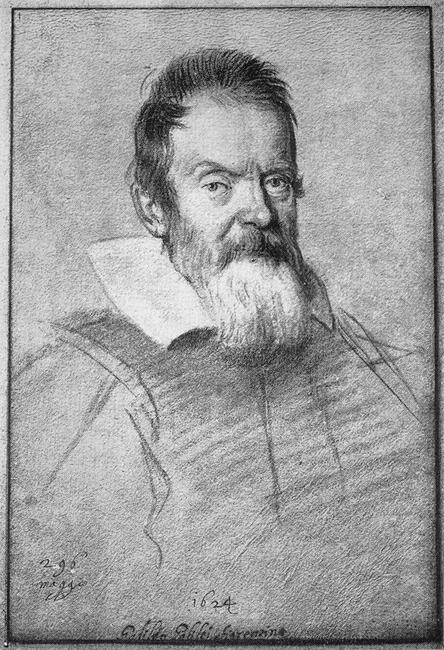
\includegraphics[width=40mm]{galileo}
\caption{Galileu Galilei}
\label{fig:galileo}
\end{figure}

\begin{figure}[hb]
\centering % Centrar a figura 
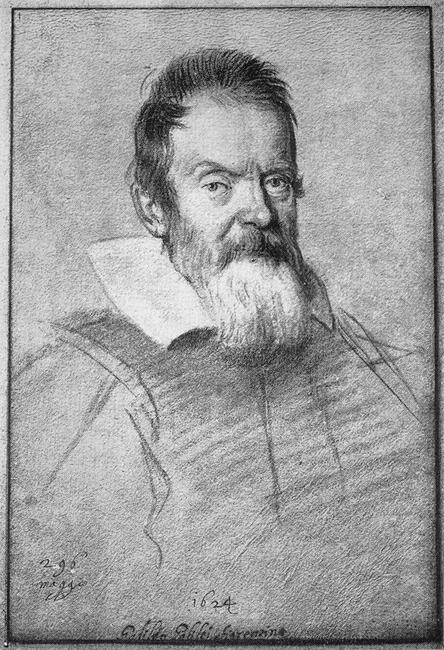
\includegraphics[width=40mm,angle=45]{galileo}
\caption{Galileu Galilei}
\label{fig:galileor}
\end{figure}

\subsection{Inserindo Tabelas}
A Tabela \ref{tab:grego}) mostra o alfabeto grego com as letras que são frequentemente utilizadas em equações matemáticas e a Tabela \ref{tab:densidades} apresenta valores de densidades de diferentes substâncias. 
  
\begin{table}[h]
\centering
\begin{tabular}{||lll|lll||}
\hline\hline
A         & $\alpha$                  & alfa    & N          & $\nu$      & niu \\ 
B         & $\beta$                   & beta    & $\Xi$      & $\xi$      & csi \\  
$\Gamma$  & $\gamma$                  & gama    & O          & o          & omicron \\
$\Delta$  & $\delta$                  & delta   & $\Pi$      & $\pi$,    $\varpi$   & pi \\  
E         & $\epsilon$, $\varepsilon$ & epsilon & P          & $\rho$,   $\varrho$  & ró \\
Z         & $\zeta$                   & zeta    & $\Sigma$   & $\sigma$, $\varsigma$ & sigma \\     
H         & $\eta$                    & eta     & T          & $\tau$     & tau \\
$\Theta$  & $\theta$, $\vartheta$     & teta    & $\Upsilon$ & $\upsilon$ & upsilon \\   
I         & $\iota$                   & iota    & $\Phi$     & $\phi$,   $\varphi$ & fi \\ 
K         & $\kappa$                  & kapa    & X          & $\chi$     & qui \\ 
$\Lambda$ & $\lambda$                 & lambda  & $\Psi$     & $\psi$,   $\varphi$ & psi \\ 
M         & $\mu$                     & miu     & $\Omega$   & $\omega$   & omega \\ 
\hline\hline 
\end{tabular}
\caption{Alfabeto grego.}
\label{tab:grego}
\end{table}

\begin{table}[ht]
\centering 
\begin{tabular}{ccl}
(a) & $[\rho]$ = & kg/m$^3$ \\
(b) & $[\rho]$ = & kg/dm$^3$ = g/cm$^3$\\
\end{tabular}\\
\ \\
\begin{tabular}{ccc}\hline\hline 
\textbf{Substância} & (a) & (b) \\ \hline\hline 
Água$^{*}$        & 1000 & 1     \\ 
Água de mar$^{*}$ & 1025 & 1,025 \\
Gelo                &  920 & 0,92  \\
Sangue              & 1050 & 1,05  \\
Alumínio            & 2710 & 2,71  \\
Ar                  & 1,29 & $1,29\times10^{-3}$ \\
Betão               & 2200 & 2,2   \\
Bronze              & 8800 & 8,8   \\
Cobre               & 8920 & 8,92  \\
Duralumínio         & 2790 & 2,79  \\ 
Glicerina$^{*}$     & 1260 & 1,26  \\ 
Granito             & 2800 & 2,8   \\ 
Eter$^{*}$          &  710 & 0,71  \\ 
Ferro               & 7840 & 7,84   \\  
Invar               & 8700 & 8,7   \\  
Irídio              & 22400 & 22,4  \\  
Latão               &  8400 & 8,4   \\ 
Mercúrio$^{*}$      & 13600 & 13,6  \\
Óleo                &   920 &  0,92 \\ 
Ouro                & 19300 & 19,3  \\ 
Petróleo            &   850 &  0,85 \\ 
Prata               & 10500 & 10,5  \\ 
Volfrâmio           & 19100 & 19,1  \\
Zinco               &  7140 & 7,14  \\ \hline\hline   
\end{tabular}\\
\ \\
$^{*}$A $20^{\circ}$C (293 K)
\caption{Densidades de diferentes substâncias.}
\label{tab:densidades}
\end{table} 

\clearpage

\subsection{Notação matemática}
Uma das maiores vantagens do \LaTeX{} é sua excelente tipografia matemática, 
vejamos como podemos inserir este tipo de notação em diferentes pontos do documento. 

\subsubsection{Expressões matemáticas no texto}
Qualquer símbolo matemático que pode ser referenciado no texto deve ser escrito entre \$ e \$. 
Por exemplo: 
a famosa equivalência entre energia e massa $E = mc^2$ escreve-se como \verb|$E = mc^2$|. 

\subsubsection{Equações}
A famosa fórmula da resolvente
\[ x_{1,2} = \frac{-b \pm \sqrt{b^2 - 4ac}}{2a} \]
escreve-se como 
\begin{verbatim}
\[ x_{1,2} = \frac{-b \pm \sqrt{b^2 - 4ac}}{2a} \]
\end{verbatim}
Se precisarmos de uma equação numerada  
\begin{equation}
\int_a^b f(x)dx = F(b) - F(a) \label{eq:integral}
\end{equation}
podemos escrever 
\begin{verbatim}
\begin{equation}
\int_a^b f(x)dx = F(b) - F(a) \label{eq:integral}
\end{equation}
\end{verbatim}
e podemos fazer-lhe referência como Eq.(\ref{eq:integral}) com o comando \verb|Eq(\ref{eq:integral})|. 
Também temos ambientes para escrever o desenvolvimento de uma expressão: 
\begin{align*}
(a+b)^2 & = (a+b)(a+b)\\
        & = a^2 + ab + ab + b^2\\
        & = a^2 + 2ab + b^2
\end{align*}
ou 
\[
\text{sgn}(x) = 
\begin{cases}
  -1 & \text{se } x < 0 \\
  \phantom{-}0 & \text{se } x = 0 \\
  \phantom{-}1 & \text{se } x > 0
\end{cases}
\]
e para anotar expressões 
\[ 
\underbrace{a^2 + b^2 = c^2}_{\text{Belo Teorema!!!}}
\]

\subsubsection{Vetores}
Podemos apresentar vetores de duas formas diferentes: 
\begin{center}
Forma ``clássica": $\vec{a}$, $\vec{b}$, $\vec{c}$... \\
Forma ``moderna": $\mathbf{a}$, $\mathbf{b}$, $\mathbf{c}$... \\
\end{center}
e se quisermos ser creativos até podemos brincar com as cores: 
\[ { \color{blue}\vec{a} } \times  {\color{blue}\vec{b} } = | { \color{blue}\vec{a} } | | { \color{blue}\vec{b} } | { \color{blue}\vec{\tau} } \]
onde $\color{blue}\vec{\tau}$ é determinado usando a regra da mão direita. 

\subsubsection{Matrizes}
O \LaTeX\ também tem comandos para mostrar matrizes (com ajuda do pacote \texttt{amsmath}): 
\[
\begin{pmatrix}
\textcolor{red}{1} & \textcolor{blue}{0} & \textcolor{green}{0} \\
\textcolor{blue}{0} & \textcolor{red}{1} & \textcolor{blue}{0} \\
\textcolor{green}{0} & \textcolor{blue}{0} & \textcolor{red}{1}
\end{pmatrix}
\quad
\text{(matriz identidade colorida com parênteses)}
\]
ou
\[
\begin{bmatrix}
\textcolor{red}{1} & \textcolor{blue}{0} & \textcolor{green}{0} \\
\textcolor{blue}{0} & \textcolor{red}{1} & \textcolor{blue}{0} \\
\textcolor{green}{0} & \textcolor{blue}{0} & \textcolor{red}{1}
\end{bmatrix}
\quad
\text{(matriz identidade colorida com colchetes)}
\]
ou 
\[
\begin{vmatrix}
\textcolor{red}{1} & \textcolor{blue}{0} & \textcolor{green}{0} \\
\textcolor{blue}{0} & \textcolor{red}{1} & \textcolor{blue}{0} \\
\textcolor{green}{0} & \textcolor{blue}{0} & \textcolor{red}{1}
\end{vmatrix}
\quad
\text{(determinante da matriz identidade colorida)}
\]

\subsubsection{Nomes de algumas funções}
Usar 
\begin{center}
\begin{tabular}{lll}
$\sin x$ & para representar o seno de $x$ & (e não o horror de $sin x$)\\
$\cos x$ & para representar o coseno de $x$ & (e não o horror de $cos x$)\\
$\tan x$ & para representar a tangente de $x$ & (e não o horror de $tan x$)\\ 
$\ln x$ & para representar o logaritmo natural de $x$ & (e não o horror de $ln x$)\\ 
$\log x$ & para representar o logaritmo de base 10 de $x$ & (e não o horror de $log x$)\\ 
$\exp(x)$ & para representar a função exponencial de $x$ & (e não o horror de $exp(x)$)\\ 
\end{tabular}
\end{center}

\section{Bibliografia} 
Há duas maneiras de organizar a bibliografia: 
\begin{itemize}
\item ``Soft'': usar um ambiente para que a bibliografia fique contida no documento. 
É funcional, mas pouco flexível. 
\item ``Hard'': organiza-se a bibliografia num ficheiro com a extensão \texttt{*.bib}, 
indica-se o nome do ficheiro no  \texttt{*.bib}, 
compila-se o \texttt{*.tex} 2 vezes, depois o \texttt{*.bib} com o bib\TeX{} e compila-se o \texttt{*.tex} mais 2 vezes. 
Este processo não é preciso quando se usa um ficheiro de estilo de uma revista. 
\end{itemize}

\label{pag:bib}
% "Soft" Bibliografia 
\begin{thebibliography}{9} % O dígito é usado para alinhar corretamente as referências. Se tiver mais do que 9 (e menos que 100) então é preferível usar {99}
\bibitem{Anjos2015} \emph{Criaçao de documentos de alta qualidade utilizando \LaTeX, uma introdução},  
António dos Anjos, ISMAT Talks, 2015. 
\bibitem{Campani2011} \emph{Introdução ao Uso do Preparador de Documentos \LaTeX}, 
Carlos A. P. Campani, UFPel/Torino, 27 de setembro de 2011. 
\end{thebibliography}
\begin{verbatim}
\begin{thebibliography}{9} 
% O dígito é usado para alinhar corretamente as referências. 
%Se tiver mais do que 9 (e menos que 100) então é preferível usar {99}
\bibitem{Anjos2015} 
\emph{Criaçao de documentos de alta qualidade utilizando \LaTeX, 
uma introdução},  
António dos Anjos, ISMAT Talks, 2015. 
\bibitem{Campani2011} 
\emph{Introdução ao Uso do Preparador de Documentos \LaTeX}, 
Carlos A. P. Campani, UFPel/Torino, 27 de setembro de 2011. 
\end{thebibliography}
\end{verbatim}

\section{Por último}
Há carateres ``proibidos'', porque são usados para indicar comandos, ambientes, etc. 
Se precisarmos dos mostrar no texto devemos usar os seguintes comandos: 
\begin{center}
\begin{tabular}{lcc}
Percentagem: & \% & \verb|\%| \\
Dolar:       & \$ & \verb|\$| \\
``É'' comercial & \& & \verb|\&| \\
Cardinal        & \# & \verb|\#| \\
Traço inferior  & \_ &  \verb|\_| \\
Barra invertida & \textbackslash &  \verb|\textbackslash| \\
Acento circunflexo: & \^{} &  \verb|\^{}| \\
Til:                & \~{} &  \verb|\~{}| \\
Chaveta para abrir: & \{ & \verb|\{| \\
Chaveta para fechar: & \} & \verb|\}| 
\end{tabular}
\end{center}

\section{Para os mais corajosos}
O \LaTeX\ até permite criar ilustrações sofisticadas, mas este é um tópico avançado. 
Quem se achar à altura do desafio pode consultar a documentação dos pacotes 
\begin{center}
\begin{tabular}{cc}
PSTricks & Tikz/PGF \\
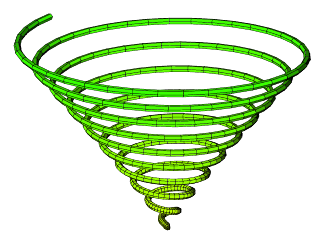
\includegraphics[height=50mm]{pstricks} & 

\includegraphics[height=50mm]{TikZGallery}
\end{tabular}
\end{center}

\end{document}
